\documentclass{article} % For LaTeX2e
\usepackage{iclr2019_conference,times}
\usepackage{caption}
\usepackage{graphicx}
\usepackage{multicol}

% Optional math commands from https://github.com/goodfeli/dlbook_notation.
\input{math_commands.tex}

\usepackage{hyperref}
\usepackage{url}
\usepackage{subcaption}
\usepackage{multirow}


\title{Reproducibility challenge: code2seq\\
\large Generating sequences from Structured Representations of Code}

% Authors must not appear in the submitted version. They should be hidden
% as long as the \iclrfinalcopy macro remains commented out below.
% Non-anonymous submissions will be rejected without review.

\author{Vegar A.~Bergum, Adam Ghoumrassi \& Nikos Angouras \\
\texttt{\{vab1g19,ag3u19,na2g16\}@soton.ac.uk}
}

% The \author macro works with any number of authors. There are two commands
% used to separate the names and addresses of multiple authors: \And and \AND.
%
% Using \And between authors leaves it to \LaTeX{} to determine where to break
% the lines. Using \AND forces a linebreak at that point. So, if \LaTeX{}
% puts 3 of 4 authors names on the first line, and the last on the second
% line, try using \AND instead of \And before the third author name.

\newcommand{\fix}{\marginpar{FIX}}
\newcommand{\new}{\marginpar{NEW}}

\iclrfinalcopy % Uncomment for camera-ready version, but NOT for submission.
\begin{document}

\maketitle

\begin{abstract}
Inspired by the reproducibility challenge encouraged by the International Conference on Representation Learning, this study attempts to contribute to the ongoing effort of addressing the lack of reproducibility of published results in Machine Learning papers. This paper aims to review the publication ‘Code2Seq: Generating Sequences from Structured Representations of Code’ by reimplementing it in a different framework, training it using the same datasets and performing a qualitative comparison of the model. The reproduced results successfully demonstrates an improvement over previous state-of-the-art results, but fail to achieve the quoted performance in the original publication.
\end{abstract}

\section{Introduction} 
Visualising the architecture of code and highlighting it's compositional paths in an abstract way can have numerous applications, including code summarization, documentation and reimplementation. Code2Seq \citep{alon2019} is a deep learning model that uses snippets of code as an abstract syntax tree (AST) to create a summary of the codes function. The model uses an encoder-decoder \citep{cho2014,sutskever2014} based approach adopted from neural machine translation (NMT) that uses attention \citep{bahdanau2015} to select the most relevant path when decoding. Using Long Short-Term Memory (LSTM) architecture, each path of the AST tree is compressed to a vector of fixed length. During the decoding stage, the model attends over another weighted average of the vector path to create each output token. In the original publication, ''code2seq: Generating sequences from structured representations of code``, an AST tree was generated for two separate tasks, in two programming languages using a model trained by four datasets of up to 16M examples. Furthermore, the model was shown to significantly outperform conventional NMT models. The Code2Seq model was initially implemented using TensorFlow, with the full source code repository\footnote{https://github.com/tech-srl/code2seq} being public.

The publication presents both a code summarization and code captioning task, where the former is based on three sets of Java source code, ranging from 700K to 16M examples. Figure \ref{fig:code-sum-vis} visualises both the captioning and summarization task. This study attempts to reproduce the F1-score obtained in the original paper on the small set of 700K samples. Due to the computational restrictions of this project and the lack of a computational cost estimates in the original publication, the smallest set was chosen to verify the results. The publication quotes a token-based F1 score of $0.432$, which is an absolute gain of $0.078$ over previous state-of-the-art methods, using this same dataset. In order to make sure that the reproduced model is unaffected by minor implementation details present in the public source-code, the re-implementation is developed using PyTorch.

\begin{figure}[hbt!]
	\centering
	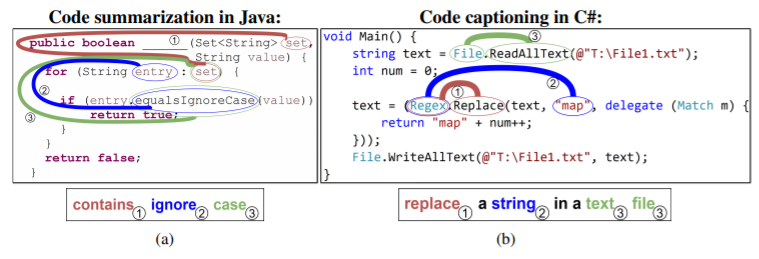
\includegraphics[width=.9\textwidth]{imgs/code_sum_cap_vis.png}
    \captionsetup{justification=centering}
	\caption{Summarization of Java and captioning in C\#, as presented in \cite{alon2019}.}
	\label{fig:code-sum-vis}
\end{figure}

%Section \ref{sec:architecture} briefly presents the model architecture, section \ref{sec:implementation} details the work and challenges related to the re-implementation and sections \ref{sec:results} presents and discusses the reproduced results.

\section{Model Architecture} \label{sec:architecture}
The Code2Seq model primarily uses the conventional encoder-decoder architecture of NMT models. Instead of reading the inputs as a flat sequence of tokens, the encoder generates a separate vector representation for each AST path. In conventional sequence to sequence models, the encoder reads an input sequence of tokens to create a large vector of fixed size. The decoder then uses the vector to generate a sequence of output tokens, thus modelling the conditional probability of the output tokens given the input tokens. On the contrary, the Code2Seq model's encoder summarises each AST path as a vector $z$, and uses the average value of all AST paths as the decoder's initial state. The decoder then generates an output sequence using attention over the encoded paths [Figure~\ref{fig:modelarch}]. During the decoding phase, a context vector $c_t$ is computed at every time step $t$ by attending over the $z$ elements using a decoding state $h_t$. The decoding state is generated using an LSTM-based RNN. A context vector $c_t$ and the decoding state $h_t$ are consequently combined to compute a prediction for each target token.
$$a^t  = softmax(h_t W_a z),\quad\quad\quad\quad\quad\quad
  c_t  = \sum_{i}^{n} a_i^t z_i$$
The AST encoder used in the Code2Seq model creates a vector representation $z_i$ of any given AST path $x_i$. The paths are made up of nodes, each equipped with a child index. The nodes are made up from a limited vocabulary of up to $364$ symbols. A bidirectional LSTM network was used to encode the paths and sub tokens were incorporated to represent the compositional nature of the value of each token. Contrary to the behaviour of conventional encoder-decoder models, the order of the input paths is not taken into account. Each path is rather encoded separately and mean pooling is used to initialise the decoder. As a result, the given input code is visualised as the summary of multiple random paths.

\begin{figure}[hbt!]
	\centering
	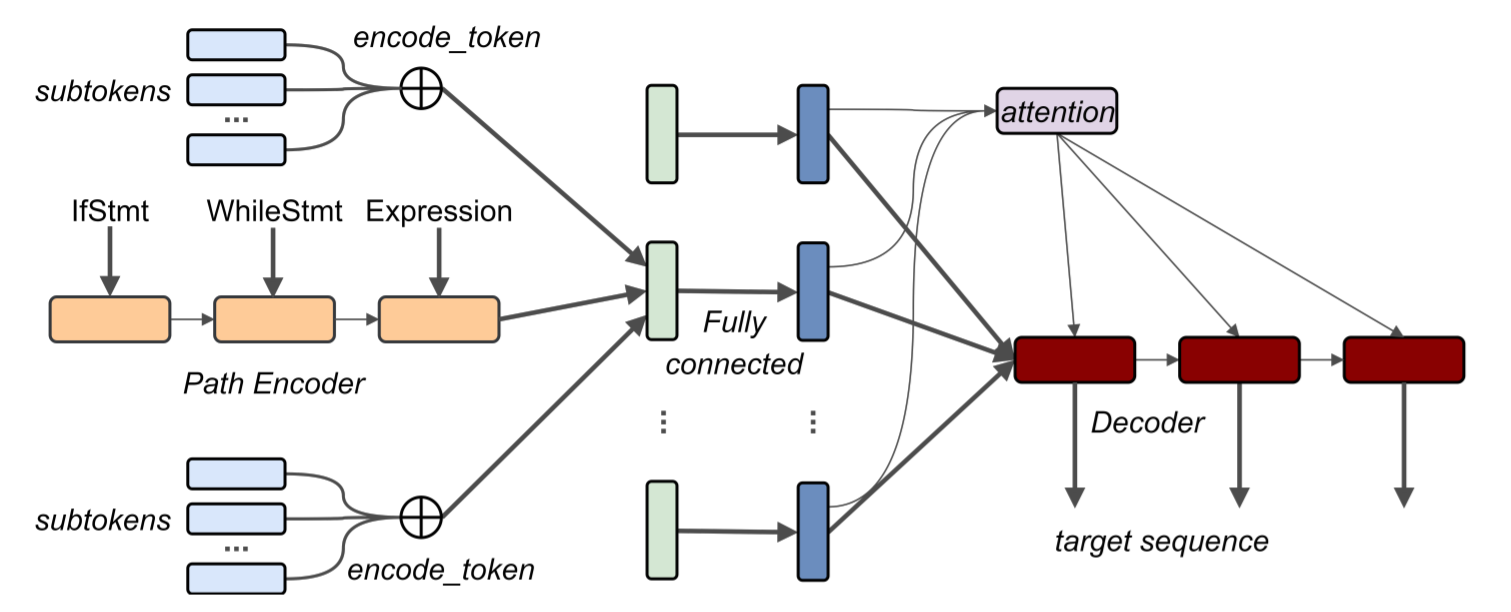
\includegraphics[width=.9\textwidth]{imgs/architecture.png}
    \captionsetup{justification=centering}
	\caption{Visualisation of Model Architecture, as presented in \cite{alon2019}.}
	\label{fig:modelarch}
\end{figure}

\section{Model Implementation} \label{sec:implementation}
Reproducing the model implementation purely based on the paper's description ended up being futile. Crucial details regarding how the encoded AST-paths and the embedded sub-tokens are concatenated into a single context tensor are omitted from the original publication. The published implementation source code, written in TensorFlow, became a required reference for certain aspects of model. 

Although the paper provides a few of the hyperparameters like learning rate, the chosen optimiser and the hidden dimensions in the LSTM-based RNNs, it fails to report embedding dimensions, dropout and batch sizes. To make the process of defining these parameters easier, the configuration setup and utility functions are ported directly from the published implementation. The configuration includes default parameters such as dropout, number of LSTM layers and embedding dimensions - all of these are assumed to be equal to the ones use to provide the final results. The utility functions include vocabulary-mapping functions and evaluation score calculations.

The use of teacher forcing during the forward training-passes of the decoder is unclear in the published implementation. In the reproduced implementation, a teacher forcing ratio of $1.0$ has been used as it is assumed to provide the highest evaluation score possible. 

\subsection{Data Loading}
To load the data efficiently into our model, we created a custom Pytorch dataset that read each item from our input file as needed, rather than loading the entire dataset into memory.
%
The input data for the loader is a preprocessed data file supplied by the authors, which contains a tokenised version of each target sequence, as well as several context sequences representing different syntactic paths through the source code. 

The main function of this module was to take the input data described above and convert this into a vector representation of the target sequence, as well as matrices containing concatenated vector representations of the start node, end node and path for each syntactic path used to predict the target sequence. These embeddings were derived using simple dictionaries that assigned each token an index value (highly infrequent tokens were given a value of 1 for “unknown”) and padding each sequence to be of identical length.
%
%In addition to the above, masking vectors and a vector of the path lengths were constructed as these are necessary for the attention mechanism used in this implementation.

One of the challenges that arose when constructing the loader was that the input file is extremely large ($691,975$ rows in the case of the training set), meaning that frequent calls to the input file created a severe bottleneck in our process. We therefore made an additional module that converted into data files into Hierarchical Data Format (HDF) which removed the need for the loader to iterate over the large input file on each read, drastically improving performance.

Unfortunately, due to time restrictions and a bug in the loader script, we were forced to abandon this module as use of this method for loading the dataset resulted in a significantly lower than state-of-the-art performance for the model (validation F1 $\sim.27$). Therefore, for the final version of this project, we instead re-purposed the data loading aspect from another PyTorch implementation of this paper found on Github from user Hukuda222%
%\footnote{https://github.com/hukuda222/code2seq}
, which significantly bolstered our performance.

\begin{figure}[hbt!]
\centering
\begin{subfigure}{.5\textwidth}
  \centering
  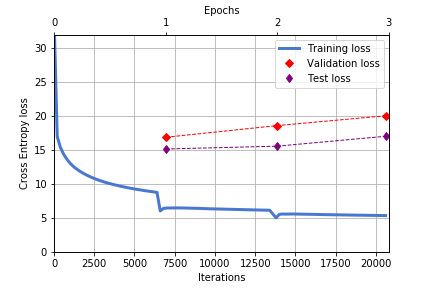
\includegraphics[width=\linewidth]{imgs/losses1.png}
  \caption{}
  \label{fig:loss}
\end{subfigure}%
\begin{subfigure}{.5\textwidth}
  \centering
  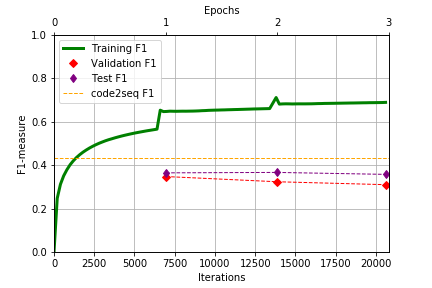
\includegraphics[width=\linewidth]{imgs/f11.png}
  \caption{}
  \label{fig:f1}
\end{subfigure}
\caption{Training history; (a) loss and (b) F1-measure.}
\label{fig:training-hist}
\end{figure}

\section{Results \& Discussion} \label{sec:results}
When training, we used the original dataset's split of 90-10 train-test and further split the training set with a 90-10 split for validation. Using the hyperparameters outlined in the paper: 2 layer bidirectional encoder LSTM with 128 units, decoder LSTM with 320 units and embedding dimensions of 128. Training with the proposed SGD optimizer with momentum and weight decay yielded very poor results from training - instead we opted to use the Adam optimizer with PyTorch's default parameters for training. We trained for $3$ epochs with a batch size of $100$. The training history is illustrated in figure \ref{fig:training-hist}. 

\setlength{\tabcolsep}{15pt}
\renewcommand{\arraystretch}{1.0}
\begin{table}[hbt!]
    \captionsetup{justification=centering}
    \caption{Code summarization results from table 1 in \cite{alon2019}, plus reproduced results. Model references have been ommitted for breivty, see original publication. All values are $\times10^2$.}
    \label{tab:results}
    \begin{center}
    \begin{tabular}{lccc}
        \hline
        \multirow{2}{*}{Model} & \multicolumn{3}{c}{Java-small}\\
        \cline{2-4}
        & Prec & Rec & F1\\
        \hline
        ConvAttention                       & 50.25 & 24.62 & 33.05\\
        Path+CRFs                           & 8.39  & 5.63  & 6.74 \\
        code2vec                            & 18.51 & 18.74 & 18.62\\
        2-layer BiLSTM (no token splitting) & 32.40 & 20.40 & 25.03\\
        2-layer BiLSTM                      & 42.63 & 29.97 & 35.20\\
        TreeLSTM                            & 40.02 & 31.84 & 35.46\\
        Transformer                         & 38.13 & 26.70 & 31.41\\
        \hline
        code2seq original & \textbf{50.64} & \textbf{37.40} & \textbf{43.02}\\
        code2seq reproduced                 & 39.70 & 33.60 & 36.40\\
        \hline
    \end{tabular}
    \end{center}
\end{table}

As is evident from the training history, the validation loss is steadily increasing after the first epoch, while its F1 score is decreasing. This is a sure sign of the model overfitting. We tested the model after each epoch, providing the best F1 score after 1 epoch, at $0.364$. Table \ref{tab:results} shows how the final results compare to the quoted Code2Seq performance, alongside other referenced models in the paper. Note that the reproduced score is lower than the quoted improvement, but higher than any of the other referenced models. 

\section{Conclusion}
In conclusion, we have re-implemented an encoder-decoder model for code-to-sequence mapping. The results show that the reproduced results demonstrate an improvement over the previous best performance (2-layer BiLSTM), but fails to achieve the quoted performance in the original publication. As the source-code for the original implementation is published and capable of achieving the quoted results, it would be sensible to assume that the re-implementation is lacking in some way. On the other hand, the reproduced results still demonstrate the publications improvement over previous state-of-the-art results on this problem.

\bibliography{references.bib}
\bibliographystyle{iclr2019_conference}

\end{document}